This section provides an overview of Project Iris, its components, and how it is intended to be used. The system will consist of an Intel RealSense SR300 camera, its driver and SDK software, and the open source code provided by Project Iris. The purpose of the system is to facilitate 3D gaze tracking for applications that do not currently have it, and to make it easier for applications in development to take advantage of 3D gaze tracking. 

\subsection{Features \& Functions}
The code provided by project Iris will include a calibration utility, an onscreen indicator of where the user is currently looking, and an API that will return the x and y coordinates of the user's current gaze position on the screen. Project Iris will be Open Source software intended for use on a Windows operating system and will require an Intel SR300.

\subsection{External Inputs \& Outputs}
Project Iris will work by using the data gathered from an Intel RealSense SR300 camera mounted as near the horizontal center and vertical top of a computer monitor as possible. The system will expect to be able to reconcile a user's eyes and facial landmarks from a distance of .2 - 1.5 meters. After a calibration procedure this data will be translated into x and y coordinates for use in other applications. In addition to the calibration utility and coordinate outputs via an API, the system will allow the developer to toggle on an indicator to visualize the current gaze position.

\subsection{Product Interfaces}
Project Iris will provide a calibration utility that will place a dot at different positions on the computer monitor (figure 2) and then use this data to output an estimate of the user's current gaze position relative to the screen. The position will be provided via an API call in the form of a pair of integers representing the estimated x and y coordinates of the user's gaze. In addition, the system will provide a toggle via the API to turn on a translucent dot that will allow for the visualization of the current estimated gaze position (figure 3).

\begin{figure}[h!]
	\centering
   	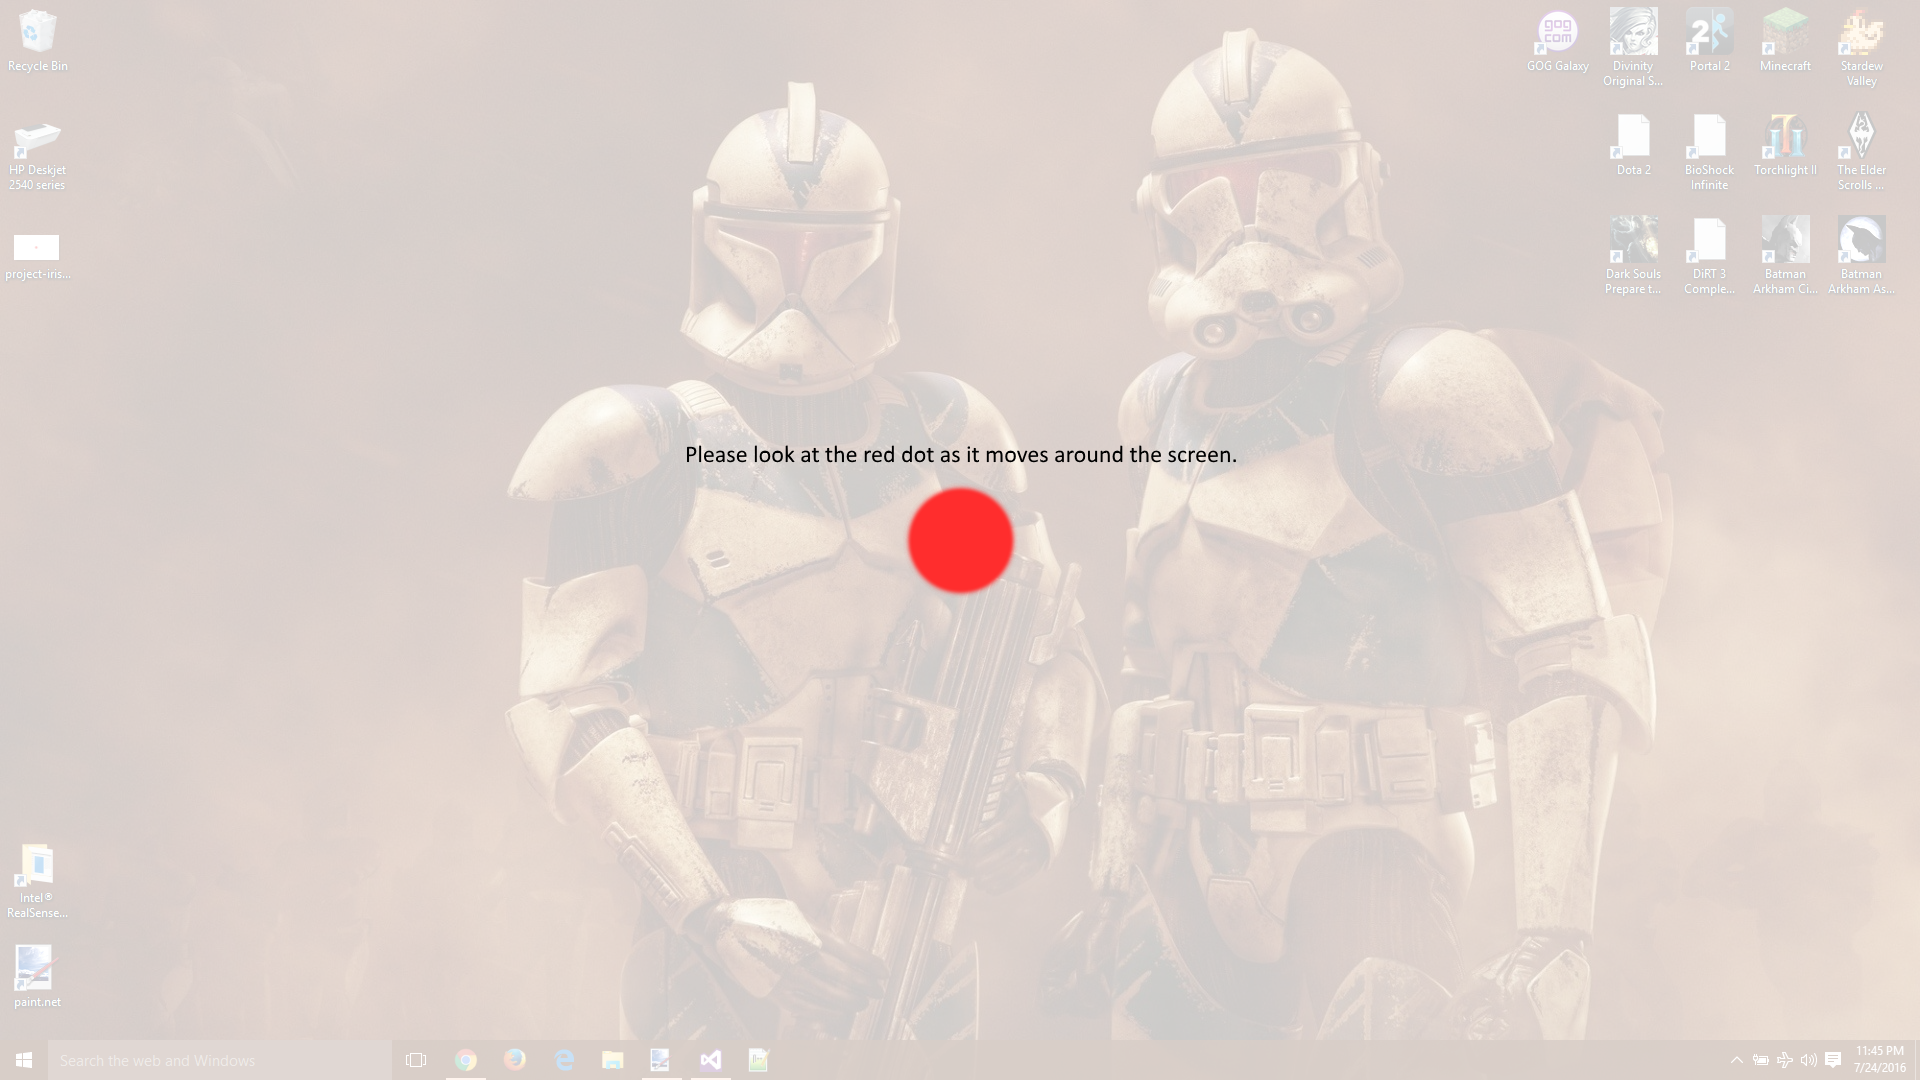
\includegraphics[width=0.60\textwidth]{images/project-iris-calibration}
    \caption{Calibration utility concept}
\end{figure}

\begin{figure}[h!]
	\centering
   	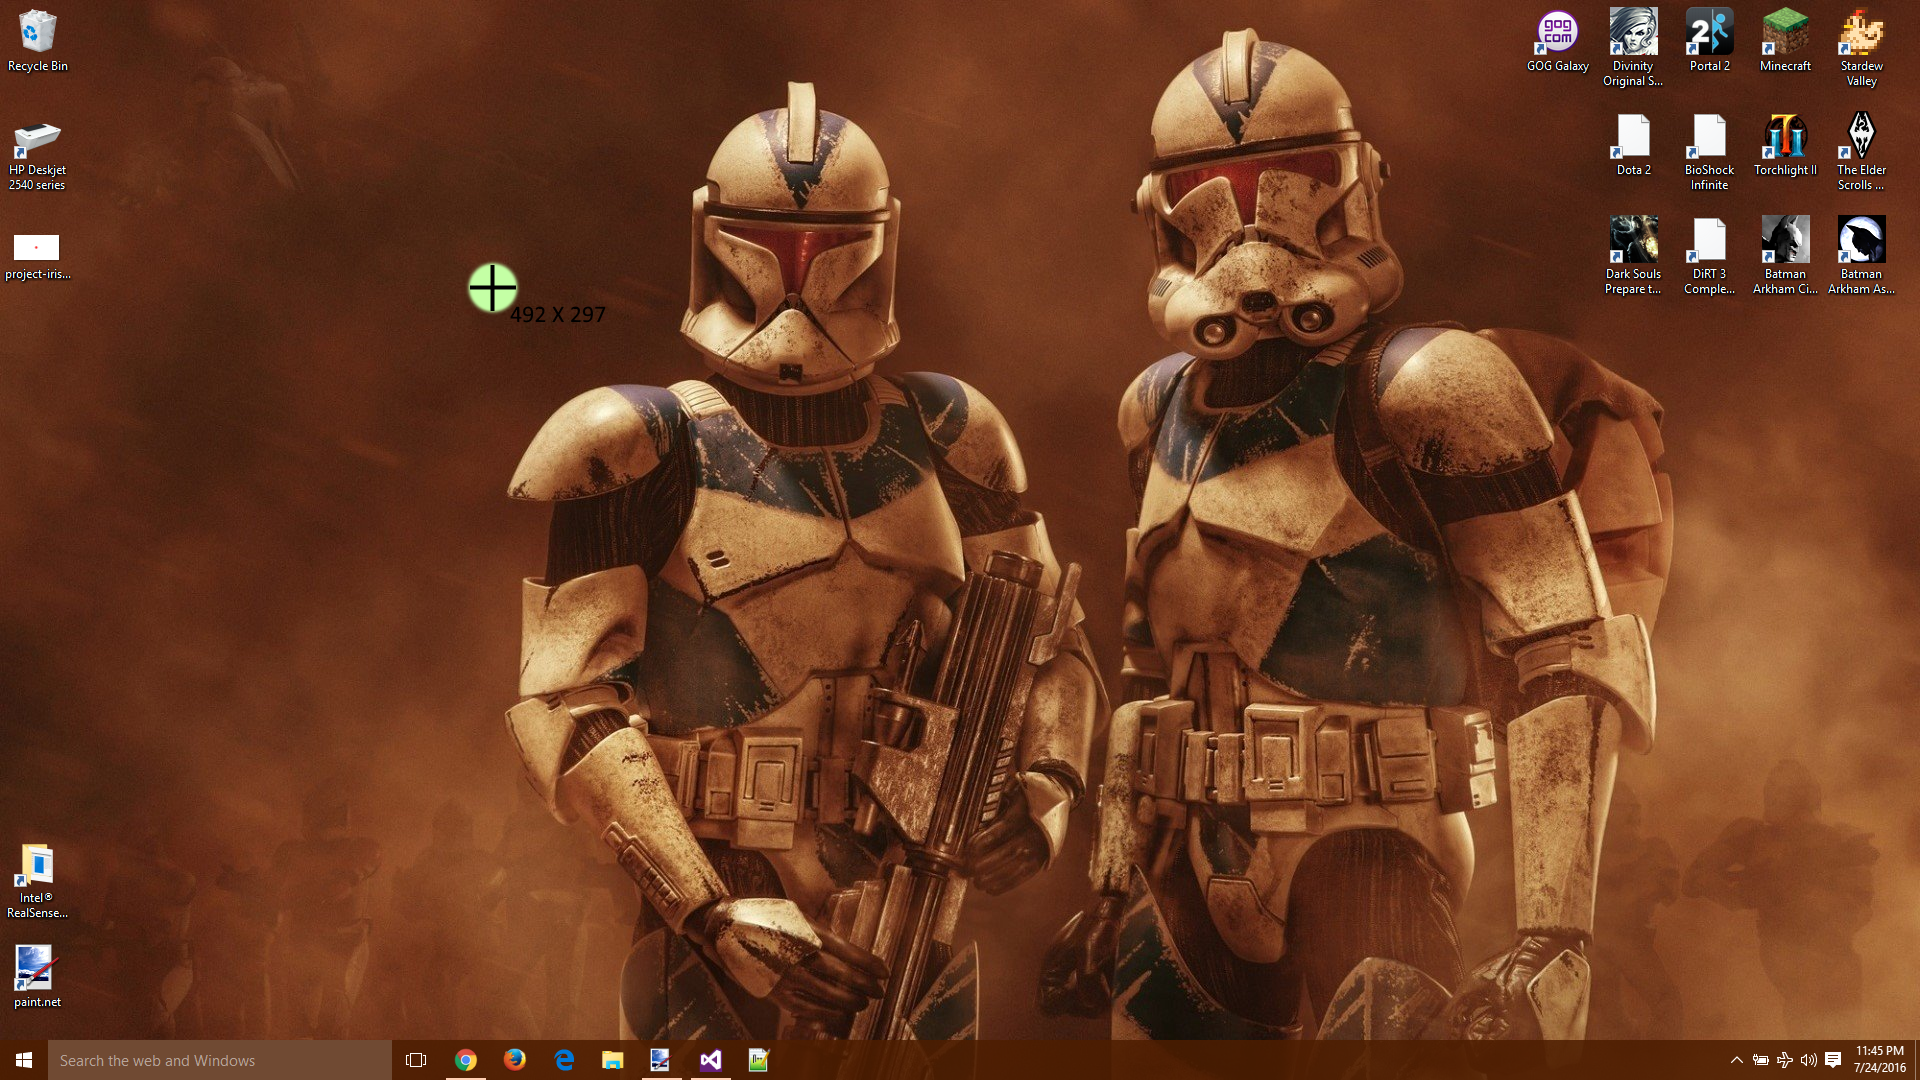
\includegraphics[width=0.60\textwidth]{images/project-iris-visualization}
    \caption{Visualization of the current gaze position concept}
\end{figure}